\chapter{Beskrivelse}
Chain of responsibility (COR) er et software pattern, der mindsker koblingen mellem sender og reciever. Princippet er, at afsenderen/klienten kun kender en abstrakt 'handler'. Handleren har en kæde af nedarvede klasser, som handleren selv sørge for at kalde rundt i kæden. 
Dette opnås ved, at der oprettes en abstrakt klasse 'Handleren'. Denne metode indeholder en abstrakt-metode til at handle et request fra klienten.
Den abstrakte-metode bliver implementeret i de konkrete handlere, der er nedarvede fra den abstrakte handler klasse.

Klassediagrammet for strukturen af COR ses i figur \ref{fig:Klassediagram}.
\begin{figure}[H]
	\centering
	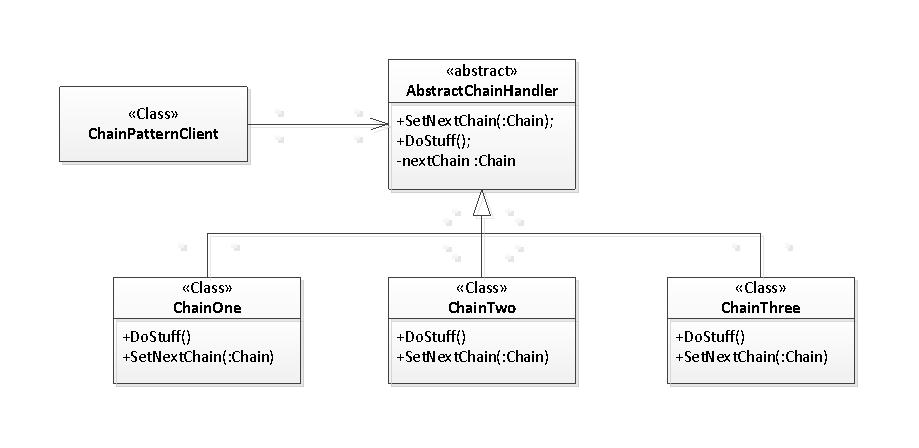
\includegraphics
	[width=140mm]{figures/UML.pdf}
	\caption{Klassediagram for Chain of Responsibility}
	\label{fig:Klassediagram}
\end{figure} 

Som det ses af klassediagramet indeholder den abstrakte klasse også metoden 'SetNextChain', der grunden til at klassen er abstrakt. Denne metode sætter, det næste led i kæden.